%%%%%%%%%%%%%%%%%%%%%%%%%%%%%%%%%%%%%%%%%%%%%%%%%%%%%%%%%%%%%%%%%%%%%%%%%%
%
% Ph.D. dissertation manuscript
%
% College of William and Mary
% Department of Physics
%
%%%%%%%%%%%%%%%%%%%%%%%%%%%%%%%%%%%%%%%%%%%%%%%%%%%%%%%%%%%%%%%%%%%%%%%%%%

\chapter{Background}
\label{chp:background}

The background material, which is necessary to understand the rest of this dissertation, is outlined in this chapter.

\section{Topic 1}
\label{sec:topic1}

This is an important topic.

\section{Topic 2}
\label{sec:topic2}

This is also an important topic.

\begin{figure} %Fig. 1                                                                                                                                                          
\begin{center}
%\hspace{12.0mm}                                                                                                                                                                
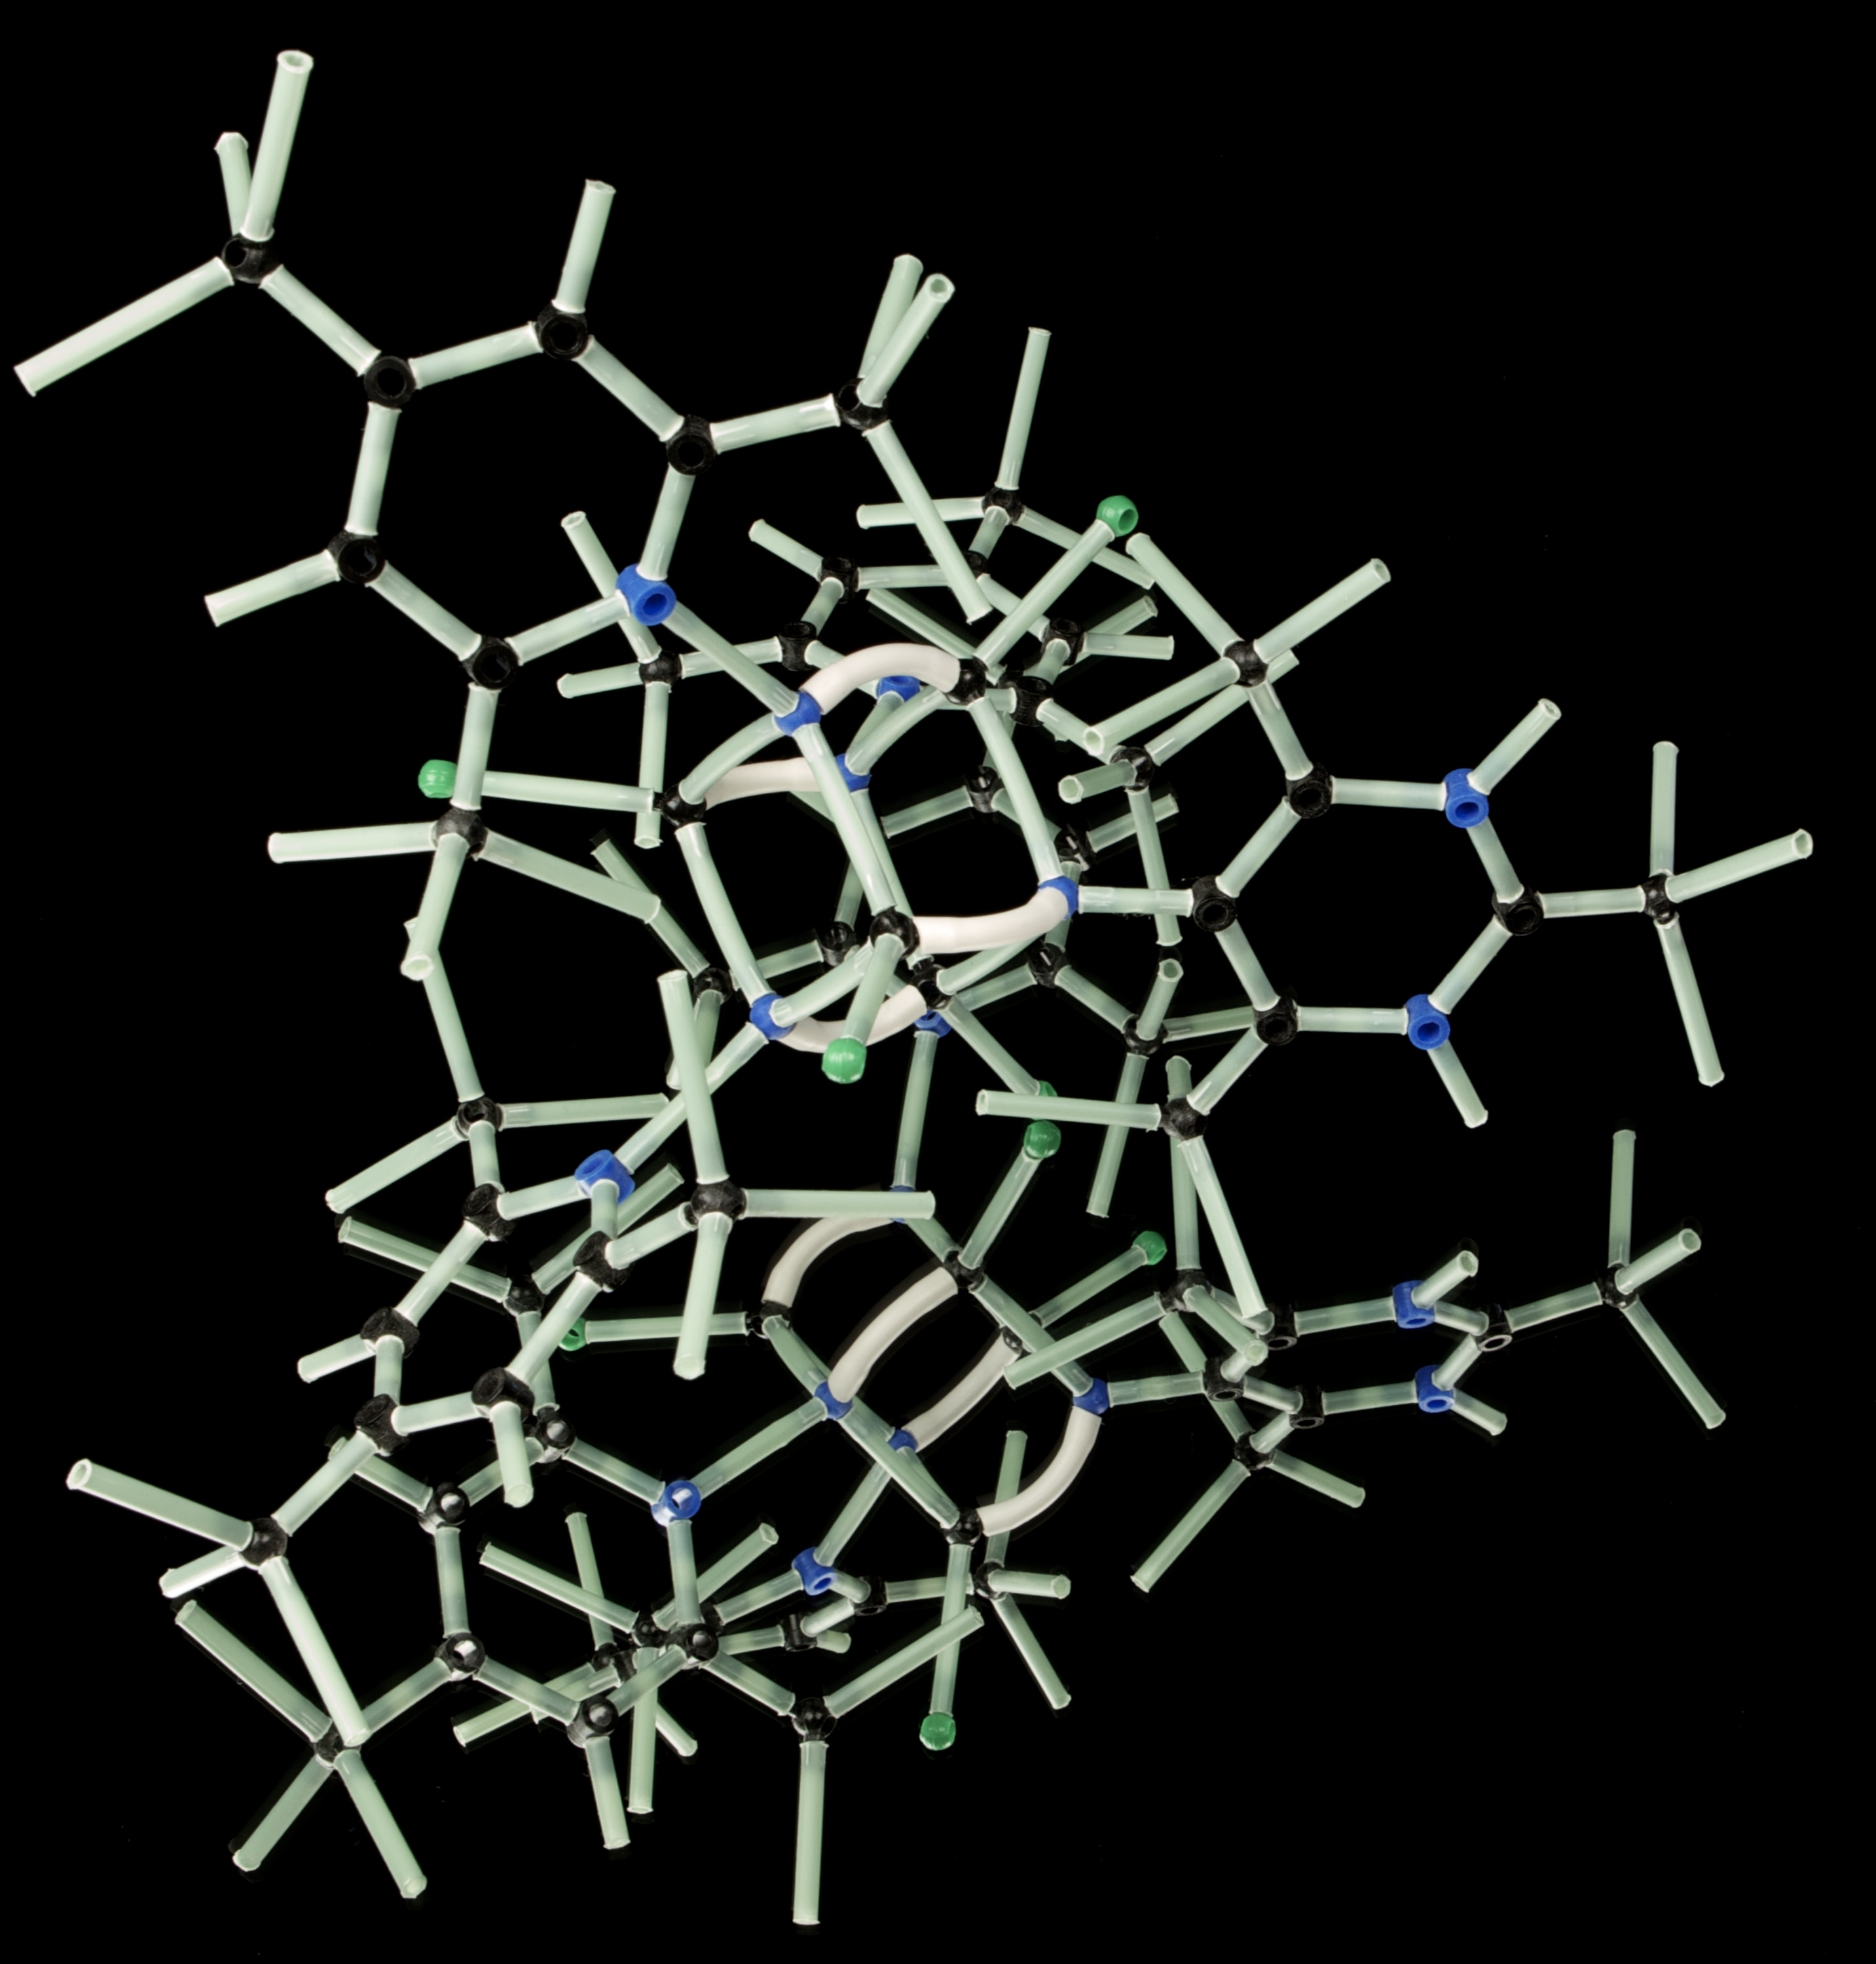
\includegraphics[width=0.6\textwidth]{figs/figure1.jpg} % use .pdf, and not .jpg. This is just an example.
\caption[a picture] % this is the short-caption that appears in the list of figures 
{\label{fig:picture}
%                                                                                                                                                                               
This is a pretty picture that helps to explain the material.
}
\end{center}
\end{figure}
